\chapter{Introduction}

%\denis

Versatile Object-oriented Toolkit for Coarse-graining Applications, or \votca, is a package which helps to systematically coarse-grain various systems. This includes  deriving the coarse-grained potentials, assessing their quality, preparing input files required for coarse-grained simulations, and analysing the latter. 

A typical coarse-graining workflow includes {\em sampling} of the system of interest, {\em analysis} of the trajectory using a specific {\em mapping} and a coarse-graining {\em method} to derive coarse-grained potentials and, in case of iterative methods, running coarse-grained simulations and iteratively {\em refining} the coarse-grained potentials.

In most cases, coarse-graining requires canonical sampling of a reference (high resolution) system. In addition, iterative methods require canonical sampling of the coarse-grained system. The sampling can be done using either molecular dynamics (MD), stochastic dynamics (SD), or Monte Carlo (MC) techniques. The latter are implemented in many standard simulation packages. Rather than implementing its own MD/SD/MC modules, \votca allows swift and flexible integration of existing  programs in such a way that sampling is performed in the program of choice. At the moment, an interface to \gromacs~\cite{gromacs4} simulation package is provided. The rest of the analysis which needed for systematic coarse-graining is done using the package tools.

\begin{wrapfigure}{ht}{4cm}
 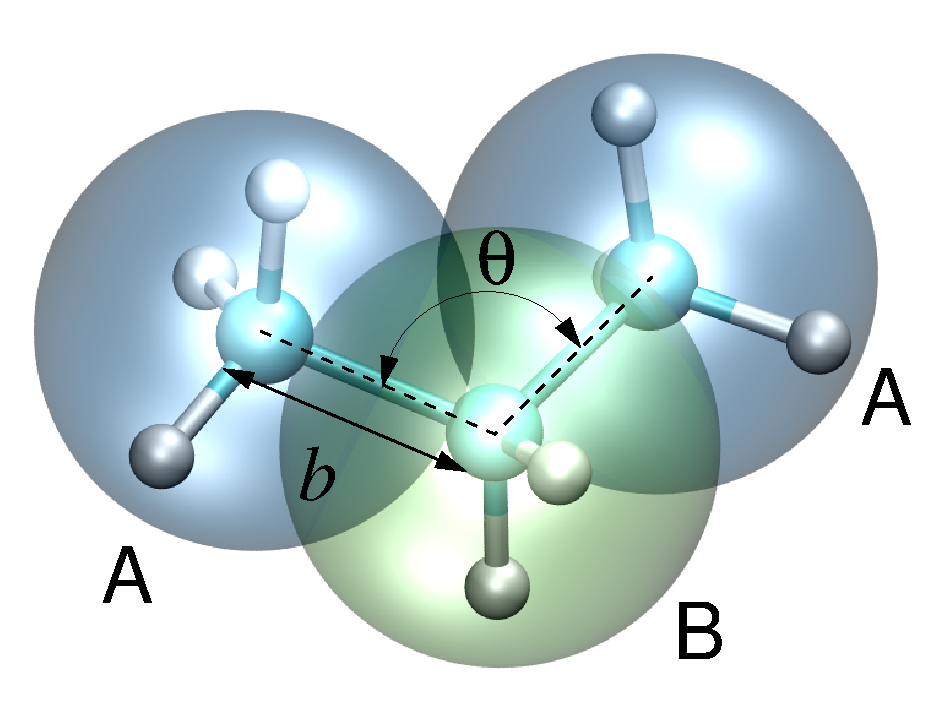
\includegraphics[width=4cm]{fig/propane}
 \caption{\small Three-bead coarse-grained model of propane.
 \label{fig:intro:propane}
}
\end{wrapfigure}

The workflow can be exemplified on coarse-graining of a propane liquid. A single molecule of propane contains three carbon and eight hydrogen atoms. A united atom coarse-grained representation of a propane molecule has three beads and two bead types, A and B, with three and two hydrogens combined with the corresponding atom, as shown in \fig{fig:intro:propane}. This representaion defines the \hyperref[sec:mapping_operator]{mapping operator}, as well as the bonded corse-grained degrees of freedom, such as the bond $b$ and the bond angle $\theta$. Apart from the bonded interactions, $u_b$ and $u_\theta$, beads belonging to different molecules have non-bonded interactions, $u_\text{AA}$, $u_\text{AB}$, $u_\text{BB}$. The task of coarse-graining is then to derive a potential energy surface $u$ which is a function of all coarse-grained degrees of freedom. Note that, while the atomistic bond and angle potentials are often chosen to be simple harmonic functions, the coarse-grained potentials cannot be expressed in terms of simple analytic functions. Instead, tabulated functions are normally used. 

The coarse-graining {\em method} defines criteria according to which the potential energy surface is constructed. For example, for the bond $b$ and the angle $\theta$  \hyperref[sec:bi]{Boltzmann Inversion} can be used. In this case a coarse-grained potential will be a potential of mean force. For the non-bonded degrees of freedom, 
\hyperref[sec:ibi]{Iterative Boltzmann Inversion (\ibi)} or \hyperref[sec:imc]{Inverse Monte Carlo (\imc)} methods can be used. In this case the radial distribution functions of the coarse-grained model will match those of the atomistic model. Alternatively, \hyperref[sec:fm]{Force Matching (\fm)} (or multiscale coarse-graining) can be used, in which case the coarse-grained potential will approximate the many-body potential of mean force. The choice of a particular method is system-specific and requires thorough consistency check. It is important to keep in mind that coarse-graining shall be used with understanding and caution, the methods should be crossed-checked with each other as well as with respect to the reference system.

More details as well as several examples can be found in ref.~\cite{Ruehle:2009.a}. Please site this paper if you are using the package. 